\documentclass[]{article}
\usepackage[margin=1.1in, portrait]{geometry}
\usepackage{amsmath}
\usepackage{amssymb}
\usepackage{amsthm}
\usepackage{mathrsfs}
\usepackage[english]{babel}
\usepackage{multirow}
\usepackage{graphicx}
\newtheorem{stel}{Stelling}
\usepackage{float}
\usepackage{textcomp}
\usepackage{footmisc}
\usepackage[colorlinks=true, urlcolor=blue, linkcolor=blue, citecolor=blue, pdfborder={0 0 0}, linktoc=page]{hyperref}
\setlength{\parindent}{0 pt}
\usepackage{etoolbox}
\usepackage{scrextend}

\newcommand{\ba}{\begin{addmargin}[9mm]{0cm}}
\newcommand{\ea}{\end{addmargin}}
\newcommand{\cm}{\color{blue} \hspace{3mm}}

\newcommand{\kb}{k_{\text{B}}}
\newcommand{\D}{\text{d}}


\title{
  \begin{figure}[H]
	   \centering
	   
\includegraphics[scale=.3]{Images/Magritte_logo_v2_BW.pdf}
  \end{figure}
  \vskip-3mm
  \textsc{\Large MAGRITTE: Multidimensional Accelerated General-purpose RadIaTive TransfEr}
  \vskip13mm
  \textsc{\Huge Background Physics}
  \vskip13mm
}

\author{\Large Frederik De Ceuster}
\date{}



\begin{document}

\maketitle

\vskip13mm

\begin{abstract}
This report aims to explain the physics behind the calculations done in the Magritte code.
\end{abstract}

\newpage

\tableofcontents

\newpage


\section{General}

Magritte\footnote{Named after Ren\'e Magritte (1898 - 1967) a Belgian surealist painter known for his playful use of light in his works. } is a multidimensional accelerated general-purpose radiative transfer code. Given a density and velocity distribution, an external radiation field and an elemental composition, it selfconsistently calculates the temperature distribution, level populations and chemical composition. Magritte is a ray-tracing code, meaning that to solve for the transport of electromagnetic radiation, the radiative transfer equation is solved along a set of rays. This is in contrast with most multidimensional radiative transfer codes which use Monte Carlo methods. Finally we should note that Magritte only solves for a state at a certain time and does not do any time evolution. However the code is written with the hope that it later will be incorporated in a full radiation hydrodynamics code.

\bigskip

The first version of Magritte is mainly based on 3D-PDR \cite{3DPDR}. The main difference between Magritte and 3D-PDR is the structure of the code and the more general treatment of the radiative transfer.  the radiative transfer is solved exactly and not in the Sobolev or large velocity gradient (LVG) approximation.
Magritte is mainly written in C with some features of C++.


\section{Assumptions and scales}


The simulations we do are characterized by a set of length-, time- and energy scales. These scales will determine which are the relevant physical processes we have to take into account. Similarly, these scales are related to the assumptions we make in our simulations.

\bigskip


We assume that the speed of light is infinite. This implies that every lightray can instantaneously influence every point on its path. This constrains the length- and timescales we can hope to simulate.

\section{Chemistry}

Given a guess for the temperature and the UV radiation field, the reaction rates are calculated. Once these are known the rate equations are evolved over a certain amount of time, starting from the initial elemental abunddances, to obtain the chemical abundances.

\begin{equation}
  \begin{cases}
  \ \dot{n}_{1} &= \ \text{formation}_{1}(n_{i}) - n_{1} \, \text{destruction}_{1}(n_{i}) \\
  \ \dot{n}_{2} &= \ \text{formation}_{2}(n_{i}) - n_{2} \, \text{destruction}_{2}(n_{i}) \\
  & \hspace{1mm} \vdots \\
  \ \dot{n}_{N} &= \ \text{formation}_{N}(n_{i}) - n_{N} \, \text{destruction}_{N}(n_{i})
  \end{cases}
\end{equation}

\section{Level populations}

The chemical abundances of all species are not enough to understand the radiative behaviour of the fluid. The radiative properties of a species depend strongly on its electron structure. The quantized electron structure gives rise to emission and absorpsion lines, i.e. strongly peaked as function of the frequency. To account for these in our description, we need to know the populaltion densities of the various energy levels of the chemical species. Usually, for computational simplicity, we will only consider the level populations of the few species yielding the strongest lines.

\subsection{Line transitions}

The dynamics of the level population densities can be described by
\begin{equation}
\frac{\partial n_{i}}{\partial t} = \nabla \cdot \left( n_{i} \textbf{v} \right) + \sum_{j=1}^{N} n_{j} R_{ji} - n_{i} \sum_{j=1}^{N} R_{ij} .
\end{equation}
The first term denotes the change in population density due to the in- or outflow of material in the parcel of space under consideration. The second term describes transitions to the level $i$ (increasing $n_{i}$) and the third term describes transitions from the level $i$ (decreasing $n_{i}$).

\bigskip

$R_{ij}$ is the transition matrix in which entry $(i,j)$ contains the transition rate from level $i$ to level $j$. The transition rates are determined by spontaneous and stimulated emission of a photon, absoption of a photon and collisional excitation and de-excitations. All these processes appear in the expression for the transition matrix through their respective Einstein coefficients
\begin{equation}
R_{ij} =
\begin{cases}  A_{ij} + B_{ij}  J_{ij} + C_{ij}   & \text{for } i>j \\
\hspace{9.5mm} B_{ij}  J_{ij} + C_{ij} & \text{for } i<j
\end{cases} .
\end{equation}
The physical meaning of the Einstein coefficients is best seen from the expressions for the change in energy caused by corresponding processes
\begin{equation}
\begin{split}
\dot{\mathcal{E}}^{\ \text{spon. em.}}_{\nu} &= \frac{h\nu_{ij}}{4\pi} \ A_{ij} \ n_{i} \phi_{\nu} \\
\dot{\mathcal{E}}^{\ \text{stim. em.}}_{\nu}  &=  \frac{h\nu_{ij}}{4\pi} \ B_{ij} \ n_{i} \ \phi_{\nu} I_{\nu} \\
\dot{\mathcal{E}}^{\ \text{abs.}}_{\nu} &=  -\frac{h\nu_{ij}}{4\pi} \ B_{ji} \ n_{j} \ \phi_{\nu} I_{\nu} \\
\end{split}
\end{equation}
The mean intensity $J_{ij}$ is defined as
\begin{equation}
J_{ij}(\textbf{x}) \equiv \oint \frac{\D \hat{\textbf{n}}}{4 \pi} \int_{0}^{\infty} \D \nu \ \phi^{(ij)}_{\nu}(\textbf{x}) \ I_{\nu}(\textbf{x},\hat{\textbf{n}}).
\end{equation}
This is the average of the radiation's specific intensity  $I_{\nu}(\textbf{x},\hat{\textbf{n}})$ over all directions and integrated over all frequencies in the line. Due to quantum effects and statistical effects there is not one frequency, but a whole profile of frequencies associated to a certain transition. The weight of each frequency is given by the line profile function $\phi^{(ij)}_{\nu}(\textbf{x})$.


\subsection{Line profiles}

Emission and absorption lines are strongly peaked as function of frequency, however they are not perfectly Dirac distributed. The line profile function $\phi_{\nu}$ describes the distribution of the line as function of frequency. The deviations from a perfect Dirac distribution are due partly to the intrisic uncerainty in the frequency of an emitted photon following Heisenberg's uncertainty relations and collisions, and partly to the thermal motions of emitting or absorbing species. The former two effects will lead to a Lorentzian profile, while the latter makes it Gaussian. In reality each effect will dominate in a different regime. This leads to a combination of a Lorentzian and Gaussian profile called the Voigt profile.

\bigskip

The Lorentzian profile is given by
\begin{equation}
L_{\nu}(\gamma) = \frac{}{}
\end{equation}


Assuming local thermodynamical equilibrium (LTE) the velocities of the particles are Maxwell-Boltzmann distributed. For one component $v_{i}$ of the velocity vector $\textbf{v}$ the distribution is
\begin{equation}
f_{\text{M.B.}}(v_{i}) = \left(\frac{m}{2\pi \kb T}\right)^{3/2} \exp\left( -\frac{m v_{i}^{2} }{2 \kb T} \right).
\end{equation}
The profile is the result of the Doppler shift caused by the above velocity distribution, hence
\begin{equation}
\phi^{(ij)}_{\nu} \ \propto \ \int_{-\infty}^{+\infty} \D v_{i} \ f_{\text{M.B.}}(v_{i}) \ \delta\left(\nu-\nu_{ij}\left(1-\frac{v_{i}}{c}\right)\right) \ = \ \exp\left( -\frac{mc^{2} (\nu-\nu_{ij})^{2} }{2 \kb T \nu_{ij}^{2}} \right).
\end{equation}
Normalizing this as distribution over frequency gives
\begin{equation}
\phi^{(ij)}_{\nu} \ = \ \frac{1}{\sqrt{\pi}\Delta\nu_{ij}} \ \exp\left( -\frac{(\nu-\nu_{ij})^{2} }{\Delta\nu_{ij}^{2}} \right),
\end{equation}
where we defined
\begin{equation}
\Delta \nu_{ij} \ \equiv \ \frac{\nu_{ij}}{c} \sqrt{\frac{2 \kb T}{m}}
\end{equation}

The Lorentzian profile is given by
\begin{equation}
L_{\nu}(\gamma) = \frac{}{}
\end{equation}

\subsubsection{Numerical evaluation of line profiles}

To calculate the level populations we need the intensity integrated over all frequencies and weighted with the line profile function. As a result we often have to evaluate integrals weighted with a Gaussian. In practice this can be done efficient using Gauss-Hermite quadrature. Gauss' quadrature theorem states that for every polynomial $p_{d}(x)$ of degree $d$, one can use the integral approximation
\begin{equation}
\int_{-\infty}^{+\infty} \D x \ \frac{e^{-x^{2}}}{\sqrt{\pi}} \ p_{d}(x) \ \approx \ \frac{2^{N-1}N!}{N^{2}} \ \sum_{n=1}^{N} \ \frac{p_{d}(x_{n})}{\big( H_{N-1}(x_{n}) \big)^{2}},
\end{equation}
where $H_{N-1}(x)$ is the (physicists') Hermite polynomial of degree $N-1$ and the $x_{n}$ are the roots  the Hermite polynomial of degree $N$. The equality is exact for polynomials of degree $d\leq2N-1$. Using this we can approximate frequency integrated intensities as
\begin{equation}
I_{ij} \ \equiv \ \int_{0}^{\infty} \D \nu \ \phi_{\nu}^{(ij)} \ I_{\nu} \ \approx \ \frac{2^{N-1}N!}{N^{2}} \ \sum_{n=1}^{N} \ \frac{ I_{ x_{n} \Delta\nu_{ij} + \nu_{ij} } }{\big( H_{N-1}(x_{n}) \big)^{2}},
\end{equation}



\subsection{Radiative transfer}

The \emph{intensity} $I_{\nu}\equiv I( \textbf{x},t;\hat{\textbf{n}},\nu)$ is defined as the energy $d\mathcal{E}$ propagated through a surface $d^{2}\textbf{S}$, in the direction $\hat{\textbf{n}}$, over a solid angle $d^{2}\omega$, within the frequency bin $[\nu,\nu+d\nu]$, in a time $dt$.
\begin{equation}
	\D \mathcal{E} \ = \ I_{\nu} \ \ \hat{\textbf{n}} \cdot \D^{2}\textbf{S} \ \D^{2}\omega \ \D\nu \ \D t
\end{equation}
For simplicity we only consider the time-independent problem. (Add figure.)

\bigskip

The \emph{radiative transfer equation} expresses how much the intensity of the electromagnetic radiation in a certain frequency bin at a certain point changes in a certain direction.
\begin{equation}
\hat{\textbf{n}} \cdot \nabla I_{\nu}(\textbf{x},\hat{\textbf{n}}) \ = \ \eta_{\nu}(\textbf{x},\hat{\textbf{n}}) - \chi_{\nu}(\textbf{x}) I_{\nu}(\textbf{x},\hat{\textbf{n}})
\end{equation}
One can see that in this equation $\eta_{\nu}(\textbf{x},\hat{\textbf{n}})$ is the \emph{emissivity} which adds to the intensity and $\chi_{\nu}(\textbf{x})$ is the \emph{opacity} of the medium, which attenuates the intensity. Note that we assumed that the opacity is independent of the direction in which we look. There are many components contributing to the emissivity and opacity.



\subsubsection{Components of the radiation field}
Next we will discuss all different components of the radiation field and how they appear in the transfer equation.

\paragraph{Lines} Electronic transitions in atoms or molecules lead to sharply peaked emissions in frequency. The corresponding emissivity and opacity of these transition can be formulated in terms of the (radiative) Einstein coefficients.
\begin{equation}
\begin{split}
\eta^{(ij)}_{\nu}(\textbf{x}) \ &= \ \frac{h \nu}{4 \pi} \ n_{i}(\textbf{x}) A_{ij} \ \phi^{(ij)}_{\nu}(\textbf{x}), \\
\chi^{(ij)}_{\nu}(\textbf{x}) \ &= \ \frac{h \nu}{4 \pi} \ \big( n_{j}(\textbf{x}) B_{ji} - n_{i}(\textbf{x}) B_{ij} \big) \ \phi^{(ij)}_{\nu}(\textbf{x}).
\end{split}
\end{equation}
Note that we make the assumption of complete redistribution by giving both the emissivity and opacity the same profile function.


\paragraph{Continuum radiation} Appart from the lines, we also consider a continuum background originating from both the cosmic microwave background (CMB) and the dust. For both we assume a Planck distribution with temperature $T_{\text{CMB}} = 2.725$ K for the CMB and for the dust we assume a local temperature field $T_{\text{dust}}(\textbf{x})$ which is calculated from the UV radiation field. Using Stefan's law, we find
\begin{equation}
\begin{split}
\eta^{\text{con.}}_{\nu}(\textbf{x}) \ &= \ \chi^{\text{con.}}_{\nu}(\textbf{x}) \big( B_{\nu}(T_{\text{CMB}}) + \nu \epsilon_{\text{dust}} B_{\nu}(T_{\text{dust}}) \big), \\
\chi^{\text{con.}}_{\nu}(\textbf{x}) \ &= \ \chi^{\text{dust}}_{\nu}(\textbf{x})
\end{split}
\end{equation}
where we used the Planck distribution
\begin{equation}
B_{\nu}(T) \equiv \frac{2 h \nu^{3}}{c^{2}} \left[ \exp\left( \frac{h \nu}{ \kb T} \right)  -1 \right]^{-1}.
\end{equation}

\paragraph{Dust scattering}
\begin{equation}
\begin{split}
\eta^{\text{sca.}}_{\nu}(\textbf{x}, \hat{\textbf{n}}) &= \chi_{\nu}^{\text{sca}}(\textbf{x}) \oint \D \hat{\textbf{n}}' \ \Phi(\hat{\textbf{n}},\hat{\textbf{n}}') I_{\nu}(\textbf{x},\hat{\textbf{n}}'), \\
\chi^{\text{sca.}}_{\nu}(\textbf{x})
\end{split}
\end{equation}
where we used the phase function  $\Phi(\hat{\textbf{n}},\hat{\textbf{n}}')$ that gives the probability for an incoming photon from direction $\hat{\textbf{n}}'$ to be scattered into direction $\hat{\textbf{n}}$.

\bigskip

Total opacity at a point is given by
\begin{equation}
\chi^{\text{tot}}_{\nu}(\textbf{x}) \ = \  \chi^{(ij)}_{\nu}(\textbf{x}) + \chi^{\text{con}}_{\nu}(\textbf{x}) + \chi^{\text{sca}}_{\nu}(\textbf{x})
\end{equation}



The total source function
\begin{equation}
S(\textbf{x}, \hat{\textbf{n}}) \ = \ \frac{1}{\chi^{\text{tot}}_{\nu}(\textbf{x})} \left( \eta^{(ij)}_{\nu}(\textbf{x}) + \eta^{\text{con.}}_{\nu}(\textbf{x}) + \eta^{\text{sca.}}_{\nu}(\textbf{x}, \hat{\textbf{n}}) \right)
\end{equation}


\subsubsection{ier solution method}

Why ier? What are the advantages compared to direct integration? Give motivation!

\bigskip

To solve the radiative transfer equation along a ray we use the ier method. The basic idea of the Feautrier method is to write the transfer equation as a second order instead of first order differential equation. Let us first make a distinction between the radiation travelling up and down a ray. Define
\begin{equation}
\begin{cases}
\ I^{+}_{\nu}(\textbf{x},\hat{\textbf{n}})  &\equiv \ I_{\nu}(\textbf{x},\hat{\textbf{n}}) \\ \\
\ I^{-}_{\nu}(\textbf{x},\hat{\textbf{n}})  &\equiv \ I_{\nu}(\textbf{x},-\hat{\textbf{n}}) .
\end{cases}
\end{equation}
Using these definitions we can introduce the new variables
\begin{equation}
\begin{cases}
\ u_{\nu}(\textbf{x},\hat{\textbf{n}})  &\equiv \ \dfrac{1}{2}\Big( I^{+}_{\nu}(\textbf{x},\hat{\textbf{n}}) + I^{-}_{\nu}(\textbf{x},\hat{\textbf{n}}) \Big) \\ \\
\ v_{\nu}(\textbf{x},\hat{\textbf{n}})  &\equiv \ \dfrac{1}{2}\Big( I^{+}_{\nu}(\textbf{x},\hat{\textbf{n}}) - I^{-}_{\nu}(\textbf{x},\hat{\textbf{n}}) \Big) .
\end{cases}
\end{equation}
The transfer equation for each of these new variables reads
\begin{equation}
\begin{cases}
\ \hat{\textbf{n}} \cdot \nabla u_{\nu}(\textbf{x},\hat{\textbf{n}}) &= \ \dfrac{1}{2} \Big( \eta_{\nu}(\textbf{x},\hat{\textbf{n}}) - \eta_{\nu}(\textbf{x},-\hat{\textbf{n}}) \Big) - \chi_{\nu}(\textbf{x}) v_{\nu}(\textbf{x},\hat{\textbf{n}}) \\ \\
\ \hat{\textbf{n}} \cdot \nabla v_{\nu}(\textbf{x},\hat{\textbf{n}}) &= \ \dfrac{1}{2} \Big( \eta_{\nu}(\textbf{x},\hat{\textbf{n}}) + \eta_{\nu}(\textbf{x},-\hat{\textbf{n}}) \Big) - \chi_{\nu}(\textbf{x}) u_{\nu}(\textbf{x},\hat{\textbf{n}}) .
\end{cases}
\label{uv}
\end{equation}
For a certain ray in direction $\hat{\textbf{n}}$ we can define the derivative along that ray and the optical depth as
\begin{equation}
\frac{\D}{\D s} \ \equiv \ \hat{\textbf{n}} \cdot \nabla \hspace{1cm} \text{and} \hspace{1cm} \D\tau_{\nu} \ \equiv \ \chi_{\nu}(\textbf{x}) \D s.
\end{equation}
By adding and subtracting the two forms of the transfer equation and substituting the results we find
\begin{equation}
\frac{\D^{2} u_{\nu}(\textbf{x},\hat{\textbf{n}})}{\D \tau_{\nu}^{2}} \ = \ u_{\nu}(\textbf{x},\hat{\textbf{n}}) - \frac{1}{2}\big( S_{\nu}(\textbf{x},\hat{\textbf{n}}) + S_{\nu}(\textbf{x},-\hat{\textbf{n}}) \big) + \frac{1}{2} \frac{\D}{\D\tau_{\nu}} \big( S_{\nu}(\textbf{x},\hat{\textbf{n}}) -  S_{\nu}(\textbf{x},-\hat{\textbf{n}}) \big) ,
\label{Feau}
\end{equation}
where the source function is defined as usual. Note that this is not the usual ier equation since we did not assume that the emissivity is isotropic. This is neded if we want to consider scattering. To elucidate the structure of this equation we can rewrite it as
\begin{equation}
\frac{\D^{2} u_{\nu}(\textbf{x},\hat{\textbf{n}})}{\D \tau_{\nu}^{2}} \ = \ u_{\nu}(\textbf{x},\hat{\textbf{n}}) - S_{\nu}^{\text{eff.}}(\textbf{x},\hat{\textbf{n}}) ,
\end{equation}


\bigskip

Now the problem is solved by discretizing $\tau_{\nu}$ and solve equation (\ref{Feau}) numerically. For simplicity, let us first consider the monochromatic case. The straightforward generalization can be found in \cite{Mihalas_s, MihalasMihalas}. Consider the discretized grid as shown in figure \ref{grid}. Note that the indices on variables now indicate optical depth points.
\begin{figure}[H]
	\centering
	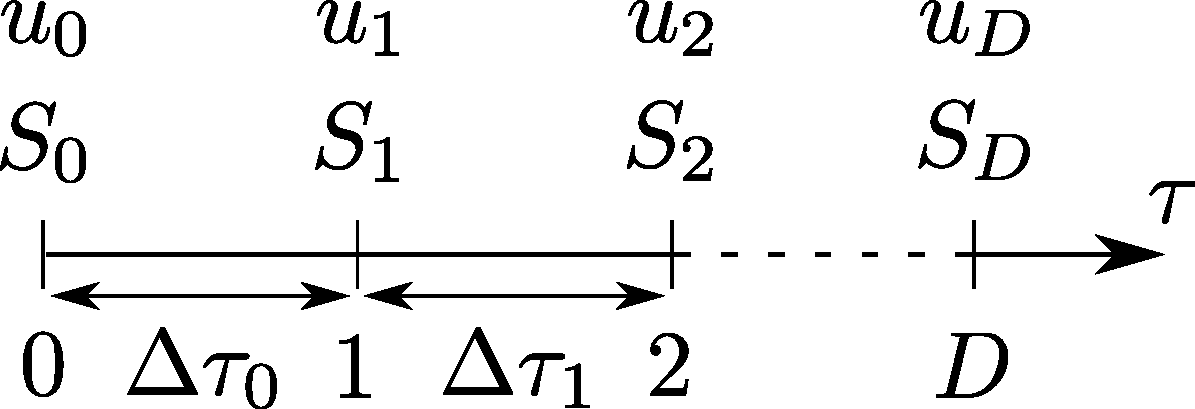
\includegraphics[scale=.3]{Images/grid.pdf}
	\caption{Discretization along the optical depth $\tau$.}
	\label{grid}
\end{figure}


Given the above discretization, the discretized version of (\ref{Feau}) then reads
\begin{equation}
\frac{\dfrac{u_{d+1}-u_{d}}{\Delta\tau_{d+1}}-\dfrac{u_{d}-u_{d-1}}{\Delta\tau_{d}}}{\dfrac{\Delta\tau_{d+1}+\Delta\tau_{d}}{2}} \ = \ - S_{d} + u_{d} .
\label{dis}
\end{equation}
The discretized equation (\ref{dis}) can be rewritten in schematic form as
\begin{equation}
-A_{d} \ u_{d-1} + B_{d} \ u_{d} - C_{d} \ u_{d+1} \ = \ S_{d},
\label{rec}
\end{equation}
where we defined
\begin{equation}
\begin{split}
A_{d} \ &\equiv \ \frac{2}{\Delta\tau_{d} (\Delta\tau_{d} + \Delta\tau_{d+1}) } , \\
C_{d} \ &\equiv \ \frac{2}{\Delta\tau_{d+1} (\Delta\tau_{d} + \Delta\tau_{d+1})} , \\
B_{d} \ &\equiv \ 1  + A_{d} + C_{d} .
\end{split}
\end{equation}
This enables us to write the descretized transfer equation in matrix form
\begin{equation}
\left( \begin{matrix}
B_{0} & -C_{0} & 0 & \cdots & 0 \\
-A_{1} & B_{1} & -C_{1} & \cdots & 0 \\
0 & -A_{2} & B_{2} & \cdots & 0 \\
\vdots & \vdots & \vdots & \ddots & \vdots \\
0 & 0 & 0 & \cdots & B_{D-1}
\end{matrix}\right)
\left( \begin{matrix}
u_{0} \\ u_{1} \\ u_{2} \\ \vdots \\ u_{D-1}
\end{matrix}\right) \ = \ \left( \begin{matrix}
S_{0} \\ S_{1} \\ S_{2} \\ \vdots \\ S_{D-1}
\end{matrix}\right)
\label{mateq}
\end{equation}
One can solve this tridiagonal matrix equation be elimination and back-substitution. One can relate the first element to the second. From the first line one can find
\begin{equation}
u_{0} \ = \ S_{0} / B_{0} \ + \ C_{0}/B_{0} \ u_{1} .
\label{init}
\end{equation}
Now one can show that it is always possible to write $u_{d}$ in terms of $u_{d+1}$ as
\begin{equation}
u_{d} \ = \ z_{d} + D_{d} \ u_{d+1}  .
\end{equation}
Substituting this in the first term of (\ref{rec}) and rewriting, one can obtain
\begin{equation}
u_{d} \ = \ \left( B_{d} - A_{d} D_{d-1} \right)^{-1} \left( S_{d} + A_{d} \ z_{d-1} \right)   + \left( B_{d} - A_{d} D_{d-1} \right)^{-1} C_{d}  \ u_{d+1}  .
\label{rec2}
\end{equation}
Now the two new coefficients can be expressed in terms of their previous values
\begin{equation}
\begin{split}
z_{d} \ &\equiv \ \left( B_{d} - A_{d} D_{d-1} \right)^{-1} \left( S_{d} + A_{d} \ z_{d-1} \right), \\
D_{d} \ &\equiv \ \left( B_{d} - A_{d} D_{d-1} \right)^{-1} C_{d} .
\end{split}
\label{elim}
\end{equation}
It is clear that to find all $u_{d}$, we first need to calculate all $D_{d}$ and $z_{d}$, to then substitute these in (\ref{rec2}) to find the $u_{d}$. The former is called the elimination step and the latter is the back-substitution step.

\bigskip

To improve the numerical behaviour of this scheme, we introduce a new variable as done in \cite{Rybicki1991}
\begin{equation}
F_{d} \ \equiv \ D_{d}^{-1} - 1.
\end{equation}
This variable allows us to rewrite the elimination step equations (\ref{elim}) as
\begin{equation}
\begin{split}
F_{d} \ &\equiv \ \left( 1 + \frac{A_{d}F_{d-1}}{1+F_{d-1}} \right) C_{d}^{-1}, \\
z_{d} \ &\equiv \ \frac{S_{d} + A_{d} z_{d-1}}{C_{d}\left(1+F_{d}\right)}.
\end{split}
\end{equation}
Note that the $F_{d}$ in the last equation is not a typo! Since every step refers to the previous one we still need an initial condition. This can be found from (\ref{init})
\begin{equation}
\begin{split}
F_{0} \ &= \ B_{0} / C_{0} - 1, \\
z_{0} \ &= \ S_{0} / B_{0}.
\end{split}
\end{equation}
Note that you do not need a final condition. Everything is defined in terms of the rows above it (and there is no mallicious $C_{D-1}$).
The mean intensity variable $u_{d}$, can now be obtained through back-substitution
\begin{equation}
u_{d} = z_{d} + \left(1+F_{d}\right)^{-1} \ u_{d+1}  .
\end{equation}
Since all variables are positive and there are no subtractions this scheme is numerically more stable.


\subsubsection{Boundary conditions}

So far, we systematically ignored boundary conditions. However in equation (\ref{mateq}) it is clear that the first and last row of the matrix do not contain the right discretized differential operator. This can be solved by imposing appropriate boundary conditions. These are given by the intensities injected in the ray, i.e. $I_{0}^{+}$ and $I_{D}^{-}$. Let us consider these to be known. The boundary conditions can be used to relate the ier variables $u$ and $v$ as, $v_{0} = I_{0}^{+} - u_{0}$ and $v_{D} = u_{D} -I_{D}^{-}$. We can use this to formulate an expression for the first and last row in the matrix equation.
One should note that the first and last row describe a relation between the first and the one to first elements of $u$, and between the last and one to last elements of $u$. Such a relation can be obtained by making a Taylor expansion from the boundary inward. For the the boundary with index 0 this yields
\begin{equation}
u_{1} \ = \ u_{0} + \Delta\tau_{0} \left.\frac{\D u}{\D \tau}\right|_{0} + \frac{1}{2} \Delta\tau_{0}^{2} \left.\frac{\D^{2} u}{\D \tau^{2}}\right|_{0} .
\end{equation}
Using equations (\ref{uv}) together with the boundary conditions on the ier variables and assuming an isotropic source function at the boundary, we obtain
\begin{equation}
u_{1} \ = \ u_{0} + \Delta\tau_{0} \left(u_{0}-I_{0}^{+}\right) + \frac{1}{2} \Delta\tau_{0}^{2} \left( u_{0} - S_{0} \right) .
\end{equation}
This can be rewritten as
\begin{equation}
\left( 1 + \frac{2}{\Delta\tau_{0}} + \frac{2}{\Delta\tau_{0}^{2}} \right)u_{0} - \frac{2}{\Delta\tau_{0}^{2}} \ u_{1}
  \ = \  S_{0} + \frac{2}{\Delta\tau_{0}} I_{0}^{+},
\end{equation}
from which we can read of the elements of the first row
\begin{equation}
\begin{split}
B_{0} \ &= \ 1 + \frac{2}{\Delta\tau_{0}} + \frac{2}{\Delta\tau_{0}^{2}}, \\
C_{0} \ &= \ \frac{2}{\Delta\tau_{0}^{2}},
\end{split}
\end{equation}
and we note that we have to add an extra term to the first element of the source term,
\begin{equation}
S'_{0}  \ = \  S_{0} + \frac{2}{\Delta\tau_{0}} I_{0}^{+}.
\end{equation}
Higher order relations can easily be obtained in a similar way. However, it turns out that second order suffices in most cases \cite{MihalasMihalas}. A similar calculation can be done for the other boundary yielding
\begin{equation}
\begin{split}
A_{D-1} \ &= \ \frac{2}{\Delta\tau_{D-1}^{2}}, \\
B_{D-1} \ &= \ 1 + \frac{2}{\Delta\tau_{D-1}} + \frac{2}{\Delta\tau_{D-1}^{2}},
\end{split}
\end{equation}
and an extra term in the last element of the source term
\begin{equation}
S'_{D-1}  \ = \  S_{D-1} + \frac{2}{\Delta\tau_{D-1}} I_{D-1}^{+}.
\end{equation}


\subsubsection{Approximate Lambda Operator}

Iteratively solving for the level populations is a notoriously slow process. The main problem is the slow convergence. To accelerate this one can use an approximate lambda operator. To construct this operator note that equation (\ref{mateq}) is of the form
\begin{equation}
\text{T} \ \textbf{u} \ = \ \textbf{S},
\end{equation}
where T is a tridiagonal matrix. Remembering the definition of  $u_{\nu}$, we can see that the inverse of T is actually the lambda operator, more precise
\begin{equation}
\textbf{u} \ = \ \text{T}^{-1} \ \textbf{S} \ = \ \frac{1}{2}\big(\Lambda^{+}_{\nu} + \Lambda^{-}_{\nu} \big) [\textbf{S}].
\end{equation}
Now we can approximate the lambda operator by taking the diagonal, or tridiagonal, or ... part of $\text{T}^{-1}$. If we use the ier method to calculate the mean intensity, there is an efficient way to calculate the approximate lambda operator at the same time \cite{Rybicki1991}.

\bigskip

We are interested in the components of the matrix $\text{L} \equiv \text{T}^{-1}$. Since $\text{T L} = \mathbb{I}$, the components satisfy
\begin{equation}
-A_{d} \ \text{L}_{d+1,p} + B_{d} \ \text{L}_{d,p}  -C_{d} \ \text{L}_{d+1,p} \ = \ \delta_{dp}.
\end{equation}
Solving this row by row from top to bottom one can obtain th recursion relations
\begin{equation}
\begin{split}
\text{L}_{d,p} &= D_{d} \text{L}_{d+1,p} + \text{Z}_{dp} \\
\text{Z}_{dp} &\equiv \left( B_{d} - A_{d} D_{d-1} \right)^{-1} \left( \delta_{dp} + A_{d} \ \text{Z}_{d-1,p} \right) \\
D_{d} &\equiv \left( B_{d} - A_{d} D_{d-1} \right)^{-1} C_{d} .
\end{split}
\label{updown}
\end{equation}
Similarly one can also obtain a set of recursion relations by solving row by row from bottom to top
\begin{equation}
\begin{split}
\text{L}_{d,p} &= E_{d} \text{L}_{d-1,p} + \text{W}_{dp} \\
\text{W}_{dp} &\equiv \left( B_{d} - C_{d} E_{d+1} \right)^{-1} \left( \delta_{dp} + C_{d} \ \text{W}_{d+1,p} \right) \\
E_{d} &\equiv \left( B_{d} - C_{d} E_{d+1} \right)^{-1} A_{d} .
\end{split}
\label{downup}
\end{equation}
Using that $\delta_{dp} = 0$ for $d\neq p$, we can find that $\text{Z}_{dp}=0$ for $d<p$ and that $\text{W}_{dp}=0$ for $d>p$. Using this in (\ref{updown}) we can obtain for the diagonal elements
\begin{equation}
\begin{split}
\text{L}_{d,d} &= D_{d} \text{L}_{d+1,d} + \text{Z}_{dd} \\
\text{L}_{d-1,d} &= D_{d-1} \text{L}_{d,d} \\
\text{Z}_{dd} &= \left( B_{d} - A_{d} D_{d-1} \right)^{-1}. \\
\end{split}
\end{equation}
Similarly for (\ref{downup}) this yields
\begin{equation}
\begin{split}
\text{L}_{d,d} &= E_{d} \text{L}_{d-1,d} + \text{W}_{dd} \\
\text{L}_{d+1,d} &= E_{d+1} \text{L}_{d,d} \\
\text{W}_{dd} &= \left( B_{d} - C_{d} E_{d+1} \right)^{-1}. \\
\end{split}
\end{equation}
One can now use both forms to obtain the diagonal elements
\begin{equation}
\text{L}_{d,d} =  \left(1-D_{d}E_{d+1}\right)^{-1}\left( B_{d} - A_{d} D_{d-1} \right)^{-1}.
\end{equation}
The off-diagonal terms can also be computed recursively using
\begin{equation}
\begin{split}
\text{L}_{d,p} &= D_{d} \text{L}_{d+1,p} \hspace{3mm} \text{for} \hspace{3mm} d<p, \\
\text{L}_{d,p} &= E_{d} \text{L}_{d-1,p} \hspace{3mm} \text{for} \hspace{3mm} d>p. \\
\end{split}
\end{equation}
From this we can construct an approximate lambda operator, e.g. by only considering the diagonal elements. This results in the local operator
\begin{equation}
\Lambda^{\ast}_{ij}(\textbf{x})[\ldots] \equiv \oint \frac{\D \hat{\textbf{n}}}{4 \pi} \int_{0}^{\infty} \D \nu \ \text{L}_{d,d},
\end{equation}
where the index $d$ relates to the position $\textbf{x}$.


\subsection{Scattering}

So far we only considered an absorption term $\chi_{\nu}(\textbf{x})$ and an emission term $\eta_{\nu}(\textbf{x},\hat{\textbf{n}})$. However, there is a third important process by which electromagnetic radiation can interact with the medium: scattering. The radiation interacts with the medium such that it is deflected. We can see this process as an absorption of radiation in a certain direction followed by emission in another direction. Note that this is why we allowed the emissivity to depend on the direction in which we look. The transfer equation including the scattering can be written as follows
\begin{equation}
\hat{\textbf{n}} \cdot \nabla I_{\nu}(\textbf{x},\hat{\textbf{n}}) \ = \ \eta_{\nu}(\textbf{x},\hat{\textbf{n}}) \ + \ \chi_{\nu}^{\text{sca}}(\textbf{x}) \oint \D \hat{\textbf{n}}' \ \Phi(\hat{\textbf{n}},\hat{\textbf{n}}') I_{\nu}(\textbf{x},\hat{\textbf{n}}') \ - \ \big( \chi_{\nu}(\textbf{x}) + \chi_{\nu}^{\text{sca}}(\textbf{x}) \big) I_{\nu}(\textbf{x},\hat{\textbf{n}}).
\label{RTEscat}
\end{equation}
The opacity gets an extra contribution from the radiation that is scattered out of the direction under consideration and the emissivity gets a contribution from the radiation of every direction that is scattered into the direction under consideration, hence the integral. $\Phi(\hat{\textbf{n}},\hat{\textbf{n}}')$ is the scattering phase function. It gives the angular distribution of the scattered radiation, i.e. the probability for incoming radiation from direction $\hat{\textbf{n}}'$ to be scattered into direction $\hat{\textbf{n}}$.

\bigskip

Including scattering in the transfer equation makes it a lot harder to solve: we need to know the radiation coming from all directions in order to solve for the radiation in a certain direction. We can overcome this difficulty by solving the equation iteratively. Let us first write equation (\ref{RTEscat}) in semi-discrete form where we only discretize the rays.
\begin{equation}
\frac{d I_{\nu}(\textbf{x},r)}{ds} \ = \ \eta_{\nu}(\textbf{x},r) \ + \ \chi_{\nu}^{\text{sca}}(\textbf{x}) \ \sum_{r' \neq r}^{N_{\text{rays}}} \Phi(r,r') I_{\nu}(\textbf{x},r') \ - \ \Big( \chi_{\nu}(\textbf{x}) + \big( 1 - \Phi(r,r) \big) \chi_{\nu}^{\text{sca}}(\textbf{x}) \Big) I_{\nu}(\textbf{x},r).
\label{RTEscat}
\end{equation}


\section{Thermal balance}

The change in the internal energy is at constant volume is determined by the temperature field. Hence one can write the change in internal energy in terms of a heating and a cooling term which are both functionals of the temperature field.
\begin{equation}
\frac{\D U}{\D t} \ \equiv \ \mathcal{F}\left[T(\textbf{x})\right]  \ = \ \mathcal{H}\left[T(\textbf{x})\right] - \mathcal{C}\left[T(\textbf{x})\right]
\end{equation}
They are functionals instead of functions because of the non-local contributions of the radiation field. The condition of thermal balance means that the internal energy is constant, or in other words that heating and cooling are equal.
\begin{equation}
\mathcal{H}\left[T_{0}(\textbf{x})\right] \ = \ \mathcal{C}\left[T_{0}(\textbf{x})\right]
\end{equation}
This condition can be used to calculate the temperature iteratively.

\bigskip

To check whether this is a valid assumption, one can check the timescale at which deviations from thermal balance are resolved. This can be found by comparing the net heating or cooling rate with the total internal energy. For a gas of simple molecules the intenral energy density of the gas can be approximated by
\begin{equation}
U \ \approx \ n \kb T ,
\end{equation}
where $n$ is the number density of the gas. Now thermal balance is a valid assumpsion if
\begin{equation}
\text{t} \ \gg \ \frac{n \kb T_{0}}{ \mathcal{F}\left[T_{0}(\textbf{x})\right] },
\end{equation}
where t is the typical timescale we can resolve.


\subsection{Dust temperature}

One can calculate the dust temperature at a certain point by assuming that the dust grains are in thermal balance with their surroundings\footnote{Check this assumption by calculating the actual heating and cooling rates to get an idea of the time scale.}. Assume spherical dust grains of radius $a$.


\subsection{Heating}

There are many heating processes contained in Magritte. The most dominant ones are the dust heating and chemical heating.
\begin{equation}
  \mathcal{H}\left[T(\textbf{x})\right] = \sum
\end{equation}

\subsection{Cooling}

For the moment the only cooling mechanism that is implemented is radiative line cooling.

\subsubsection{Radiative line cooling}

A gas can (locally) cool by radiative cooling when radiation from a certain region can escape i.e. the radiation is emitted by a region but not absorbed in that same region. The emission can be either spontaneous or stimulated.

\bigskip

The rate of energy emission in a frequency bin $\nu_{ij}$ can be given by
\begin{equation}
\dot{\mathcal{E}} \ = \ \dot{\mathcal{E}}_{\text{spontaneous emission}} + \dot{\mathcal{E}}_{\text{stimulated emission}} - \dot{\mathcal{E}}_{\text{absorption}} .
\end{equation}
The last term is needed because the stimulated emission will be counter acted by absoption. Using the definitions of the Einstein coefficients we can rewrite this as
\begin{equation}
\dot{\mathcal{E}} \ = \ h\nu_{ij} \ \phi_{\nu} \Big( A_{ij} \ n_{i}  + J_{\nu} \left( B_{ij} \ n_{i} - B_{ji} \ n_{j} \right) \Big).
\end{equation}
In terms of the line source function $S_{ij}$ the result can be written slightly more compact
\begin{equation}
\dot{\mathcal{E}} \ = \ h\nu_{ij} \ A_{ij} \ n_{i}  \phi_{\nu} \left( 1  - \frac{J_{\nu}}{S_{ij}} \right).
\end{equation}
The total radiative cooling is giver by the expression above for every downward transition i.e.
\begin{equation}
\dot{\mathcal{E}} \ = \ \sum_{j} \sum_{i>j} h\nu_{ij} \ A_{ij} \ n_{i}  \phi_{\nu} \left( 1  - \frac{J_{\nu}}{S_{ij}} \right).
\end{equation}
This is the way in which the radiative cooling is implemented in the code (\texttt{cooling.cpp}). Since we only consider radiative cooling at the moment, the cooling functional is
\begin{equation}
\mathcal{C}\left[T(\textbf{x})\right] = \dot{\mathcal{E}}
\end{equation}


\section{Applications}

\subsection{Composite galaxies}

\subsubsection{Parameter space}

\begin{tabular}{ l | l | l}
  \textit{parameter} & \textit{min.} & \textit{max.} \\ \hline
  $n_{H}$            & $10^2$        & $10^4$ \\
\end{tabular}



\subsection{Stellar winds}

\subsection{Supernova remnants}

\subsection{CMB cosmology}



\newpage

\appendix

\section{3D-PDR}

\subsection{Sobolev approximation}

The main difference between 3D-PDR and the first version of Magritte is that former used the Sobolev approximation.


\newpage

\bibliography{library}
\bibliographystyle{ieeetr}



\end{document}
